% Define block styles
\tikzstyle{block} = [draw, rectangle, text centered, text width=10em, minimum height=0.5em, rounded corners=true]
\tikzstyle{background} = [draw, rectangle, text centered, text width=3.5cm, minimum height=3.5cm, color=white]
\tikzstyle{arrowtext} = [text width=4em, text centered]
\tikzstyle{arrow} = [draw, -latex]

\definecolor{red1}{RGB}{160,0,0}
\definecolor{green1}{RGB}{0,160,0}
\definecolor{blue1}{RGB}{0,0,160}

\usetikzlibrary{shapes.geometric,arrows,positioning,calc,patterns,angles,quotes}

	      
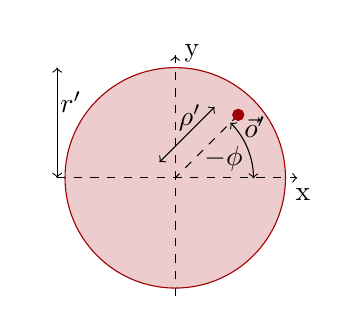
\begin{tikzpicture}[node distance=4em, auto]
    % Background size
    \node[background] at (0,0.15cm) {};

    % circle
    \draw[red1, fill=red1!20] (0,0) circle (1.4);

    % Draw axis
    \draw [->, dashed] (-1.5,0) |- (1.55,0) node [xshift=0.2em, yshift=-0.6em] {x};
    \draw [->, dashed] (0,-1.5) |- (0,1.55) node [xshift=0.6em, yshift=0.1em] {y};
    \draw [-, dashed] (0.8,0.8) -- (0,0);

    % point
    \draw[fill=red1, color=red1] (0.8,0.8) circle (2pt) node [below, color=black, xshift=0.6em, yshift=0.1cm] {$\vec o'$};

    % sizes
    \path[<->]
        (-1.5,0.0) edge node [xshift=0.5em, yshift=0.75em, anchor=center] {$r'$} (-1.5,1.4)
        (-0.2,0.2) edge node [xshift=0.1em, yshift=0.6em, anchor=center] {$\rho'$} (0.5,0.9);

    % angles
    \draw[black, fill=none, <->] (0.7,0.7) arc (45:0:1) node [xshift=-0.38cm, yshift=0.25cm] {$-\phi$};
\end{tikzpicture}
